% Пример заготовки для презентации с использованием класса Beamer LaTeX.
% Версия от 09 ноября 2018 года.
\documentclass[12pt,a4paper,mathserif]{beamer}
\usepackage[utf8x]{inputenc}
\usepackage{ucs}
\usepackage[T2A]{fontenc}
\usepackage[english,russian]{babel}
\usepackage{amsmath}
\usepackage{amsfonts}
\usepackage{amssymb}
\usepackage{mathtext}
\usepackage{graphicx}
\usepackage{enumerate}
\usepackage{multirow}
\usepackage{ragged2e}
% Пакет для оформления исходного кода
\usepackage{minted}
\usepackage{adjustbox}
\justifying
\renewcommand{\raggedright}{\leftskip=0pt \rightskip=0pt plus 0cm}
\setbeamertemplate{caption}[numbered]

\usetheme {Madrid}
\usecolortheme [RGB={85, 107, 47}]{structure} %Dark Olive Green

\author[Лаптев А.В.]{{Cтудент 595 группы: Лаптев А.~В.}\\
{Научный руководитель: Шмаков И.~А.}}
\title[Барнаул 2023]{Проектирование и разработка устройства для генерации персонажа D\&D}
% \subtitle{Отчет по научно-исследовательской работе}

\begin{document}
\begin{frame}
\maketitle
\end{frame}

\begin{frame}{Актуальность}
    \setlength{\parindent}{0.5cm}
    На сегодняшний день D\&D является, пожалуй, самой популярной стратегией, которая собрала вокруг себя огромное сообщество игроков.

    Для игры в эту настольную ролевую игру каждый игрок должен создать своего персонажа с определенными навыками и характеристиками. Создание персонажа довольно длительный и кропотливый процесс, требующий знания правил игры, которые довольно обширны. Данное устройство нужно для того, чтобы облегчить игрокам, в особенности начинающим, генерацию их игрового персонажа и выполнять большинство расчетов игровых характеристик вместо игроков.
    
    Для D\&D разработано огромное количество Web-ресурсов и ботов от энтузиастов и крупных компаний, которые облегчают игрокам процесс игры и генерации своего персонажа.
\end{frame}

\begin{frame}{Цель и задачи работы}
    \setlength{\parindent}{0.5cm}
    Целью работы является: спроектировать и разработать портативное устройство для генерации персонажа D\&D, которое будет приспособлено для повседневного использования в любом месте без подключения к Интернету.

    Задачи, которые необходимо решить для достижения цели:

    \begin{enumerate}
        \item подбор компонентов, необходимых для прототипирования;
        
        \item проектирование функциональных возможностей приложения;
        
        \item реализация в программном коде алгоритмов согласно базовым правилам D\&D5;
        
        \item отладка и тестирование работоспособности программной и аппаратной части прототипа устройства;
        
        \item сборка прототипа устройства.
    \end{enumerate}
\end{frame}

\begin{frame}{Функционал генератора персонажей}
    \setlength{\parindent}{0.5cm}
    Необходимый функционал, реализованный в данном генераторе персонажей:

    \begin{enumerate}
        \item выбор расы персонажа;
    
        \item выбор класса персонажа;
    
        \item генерация значений 5 базовых характеристик:
    
        \begin{enumerate}
            \item сила (strong --- сокращенно <<Str>>);
            
            \item телосложение (constitution --- сокращенно <<Con>>);
            
            \item ловкость (dexterity --- сокращенно <<Dex>>);
            
            \item интеллект (intelligence --- сокращенно <<Int>>);
            
            \item мудрость (wisdom --- сокращенно <<Wis>>);
            
            \item харизма (charisma --- сокращенно <<Cha>>).
        \end{enumerate}
    
        \item расчет значений для ряда побочных характеристик: класс защиты и хит-поинтов персонажа (на основе базовых характеристик).
    
        % \item Выбор снаряжения на основе ранее выбранных игроком характеристик;
    
        % \item Еще некоторые побочные характеристики.
    \end{enumerate}
\end{frame}

\begin{frame}{\smallПодбор аппаратной части. Выбор отладочной платы}
    \tiny
    \begin{minipage}{0.5\linewidth}
    ATmega328:
    \begin{itemize}
        \item микроконтроллер: ATmega328;
        \item тактовая частота: 16 МГц;
        \item напряжение логических уровней: 5 В;
        \item входное напряжение питания: 7-12 В;
        \item порты ввода-вывода общего назначения: 20;
        \item максимальный ток с пина ввода-вывода: 40 мА;
        \item максимальный выходной ток пина 3.3V: 50 мА;
        \item максимальный выходной ток пина 5V: 800 мА;
        \item порты с поддержкой ШИМ: 6;
        \item порты с АЦП: 6;
        \item разрядность АЦП: 10 бит;
        \item flash-память: 32 КБ;
        \item EEPROM-память: 1 КБ;
        \item ОЗУ: 2 КБ;
        \item размеры: 69×53 мм.
    \end{itemize}
    \end{minipage}
    \hfill
    \begin{minipage}{0.5\linewidth}
    Xtensa LX6:
    \begin{itemize}
        \item микропроцессор: двухядерный 32-бит Xtensa LX6;
        \item тактовая частота: 160-240 МГц;
        \item напряжение логических уровней: 3,3 В;
        \item входное напряжение питания: 5-14 В;
        \item порты ввода-вывода общего назначения: 10;
        \item максимальный ток с пина ввода-вывода: 12 мА;
        \item максимальный выходной ток пина 3.3V: 1 А;
        \item порты с поддержкой ШИМ: 16;
        \item порты с АЦП: 18;
        \item разрядность АЦП: 12 бит;
        \item flash-память: 448 КБ;
        \item ОЗУ: 520 КБ;
        \item беспроводная связь: Wi-fi 802.11 b/g/n 2.4 Гц (до 150 Мбит/сек);
        \item Bluetooth: v4.2 BR/EDR and BLE;
        \item размеры: 51x28 мм.
    \end{itemize}
    \end{minipage}
\end{frame}

\begin{frame}{\smallПодбор аппаратной части. Выбор периферии}
    \scriptsize
    \begin{minipage}{0.5\linewidth}
    1602 LCD Keypad Shield:
    \begin{itemize}
        \item цвет подсветки: синий;
        \item количество символов в строке: 16;
        \item количество строк: 2;
        \item язык: латиница;
        \item совместимость с Arduino Uno;
        \item напряжение питания: 5 В;
        \item тип матрицы дисплея: LCD;
        \item 5 кнопок для управления и кнопка сброса.
    \end{itemize}
    \end{minipage}
    \hfill
    \begin{minipage}{0.5\linewidth}
    LCD-дисплей:
    \begin{itemize}
        \item цвет подсветки: синий;
        \item количество символов в строке: 16;
        \item количество строк: 2;
        \item язык: латиница;
        \item для подключения необходима макетная плата;
        \item напряжение питания: 5 В;
        \item тип матрицы дисплея: LCD.
    \end{itemize}
    Кнопки:
    \begin{itemize}
        \item 5 кнопок для управления и кнопка сброса;
        \item для подключения необходима макетная плата.
    \end{itemize}
    \end{minipage}
\end{frame}

\begin{frame}{Внешний вид устройства}
    \begin{figure}[H]
        \begin{minipage}[h]{0.45\linewidth}
            \center{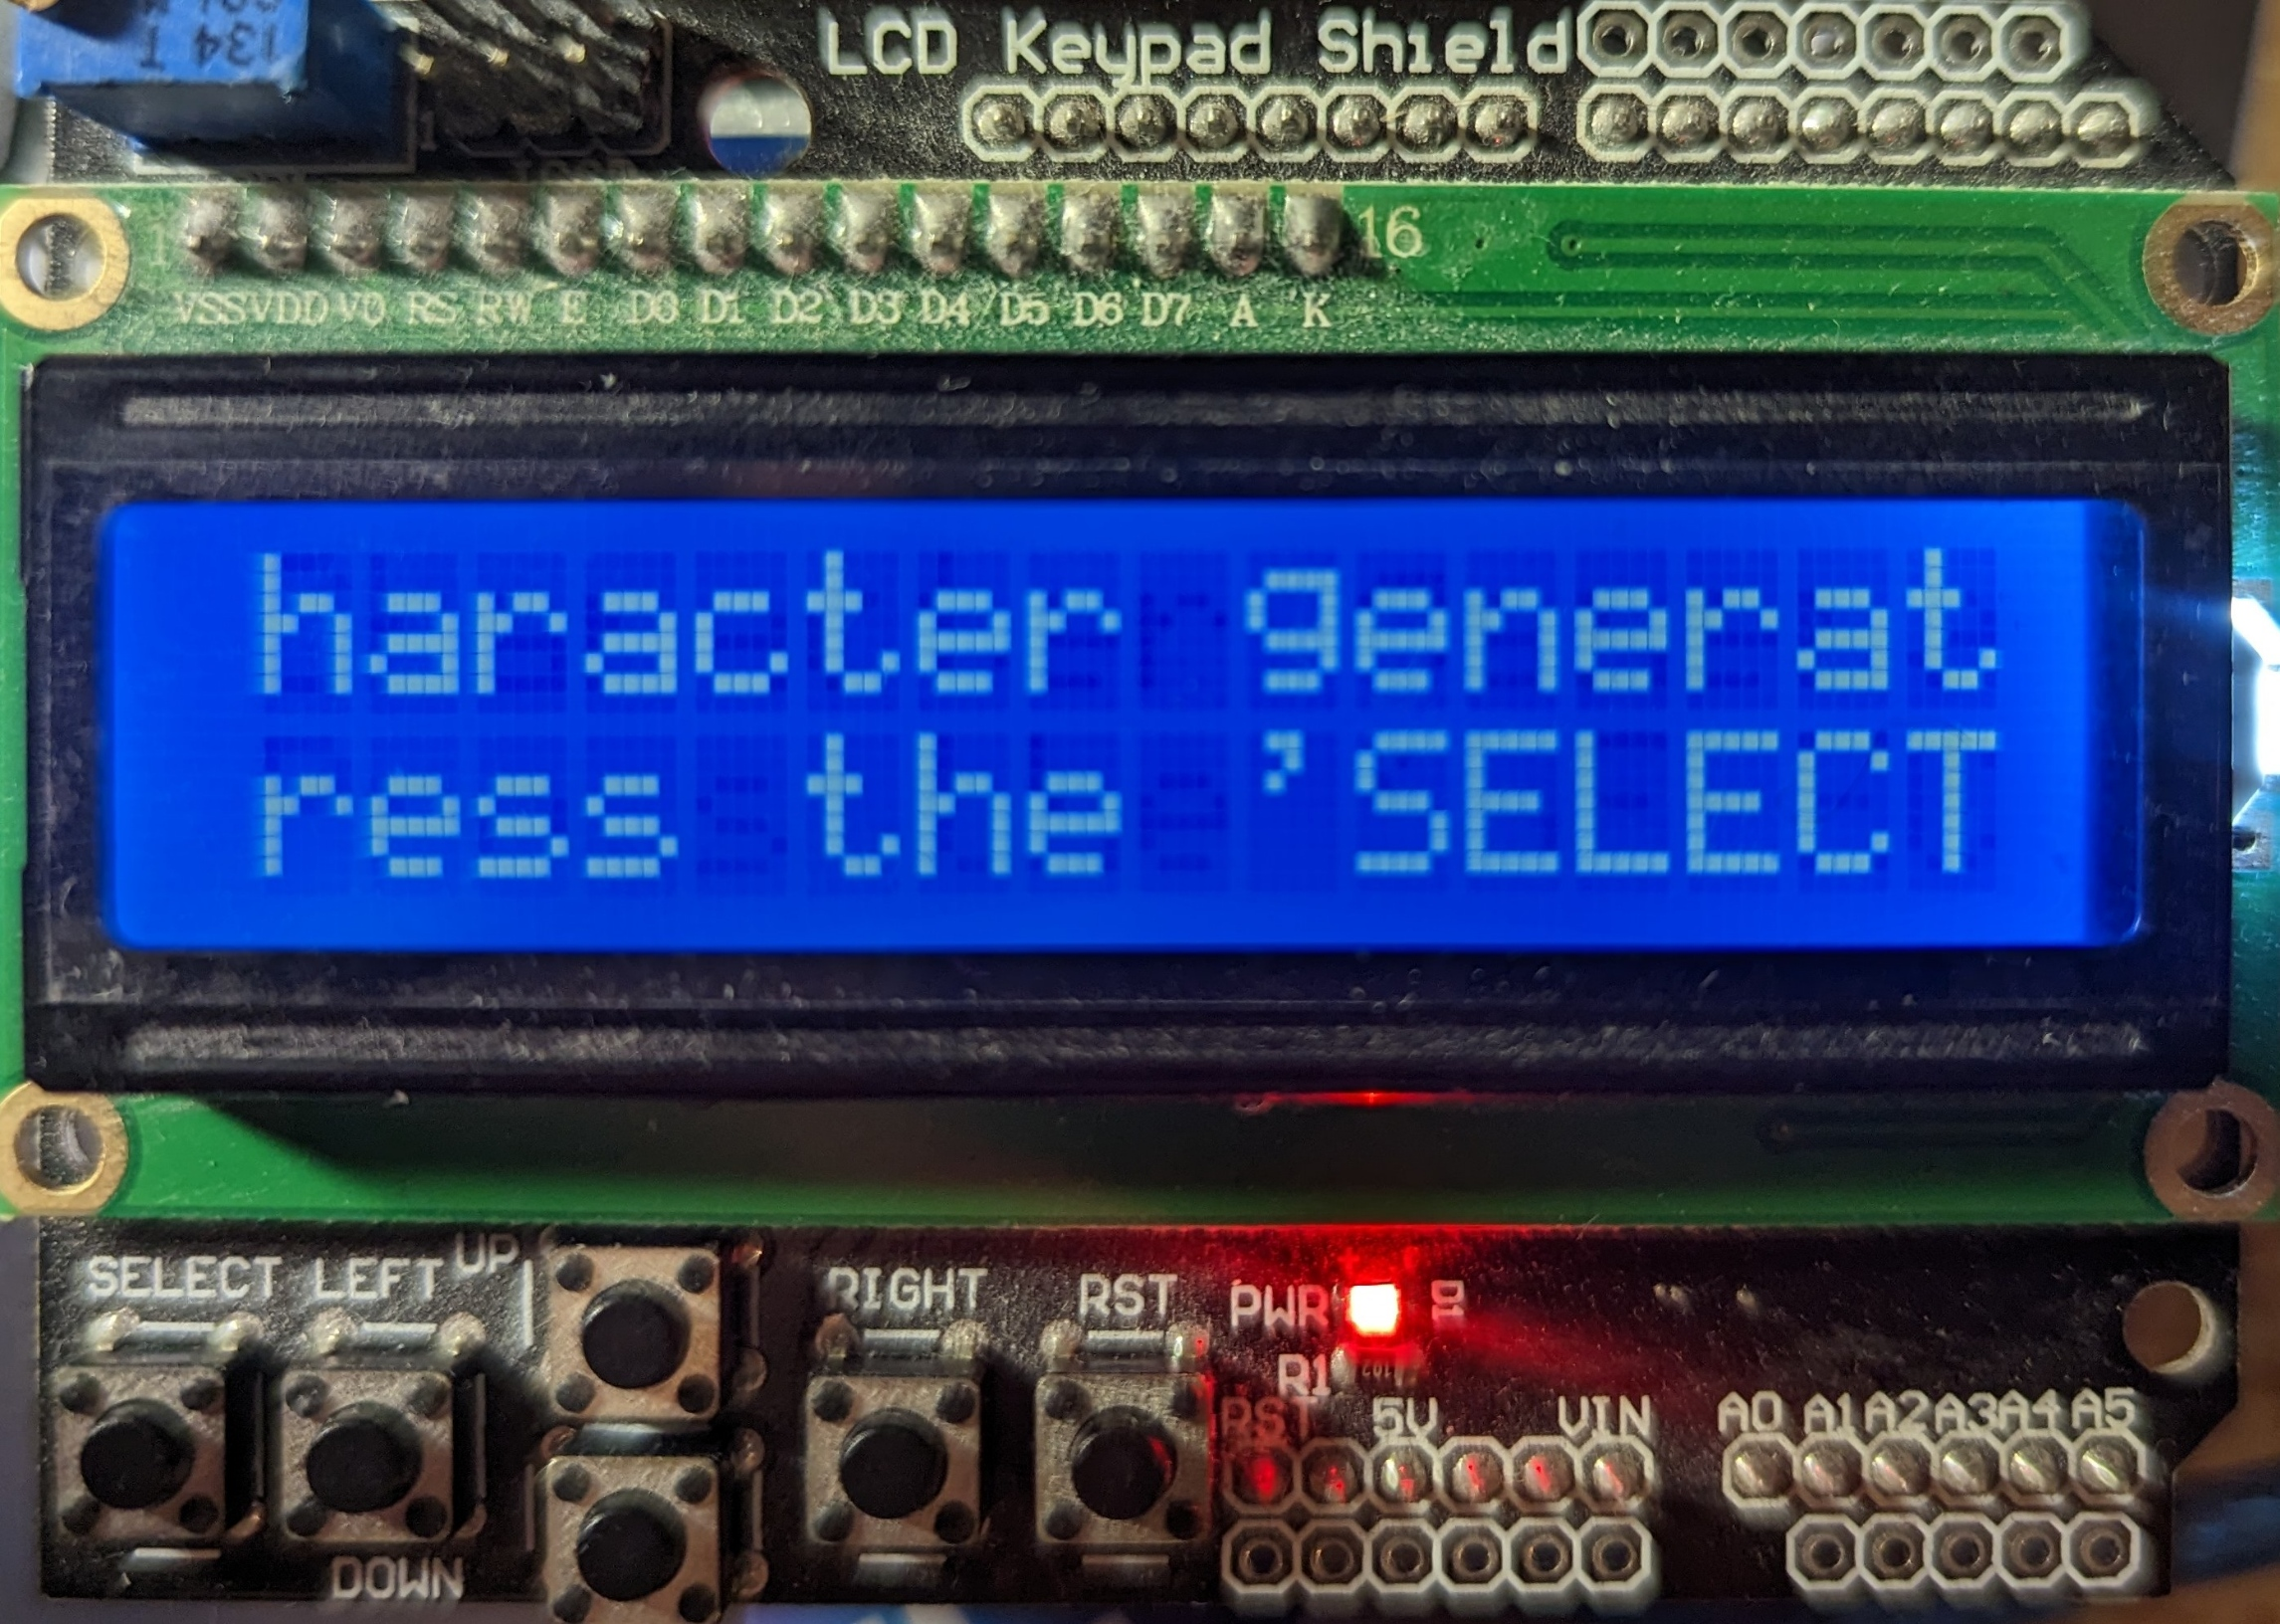
\includegraphics[width=1\linewidth]{mainWindow.jpg}} \\
        \end{minipage}
        \hfill
        \begin{minipage}[h]{0.45\linewidth}
            \center{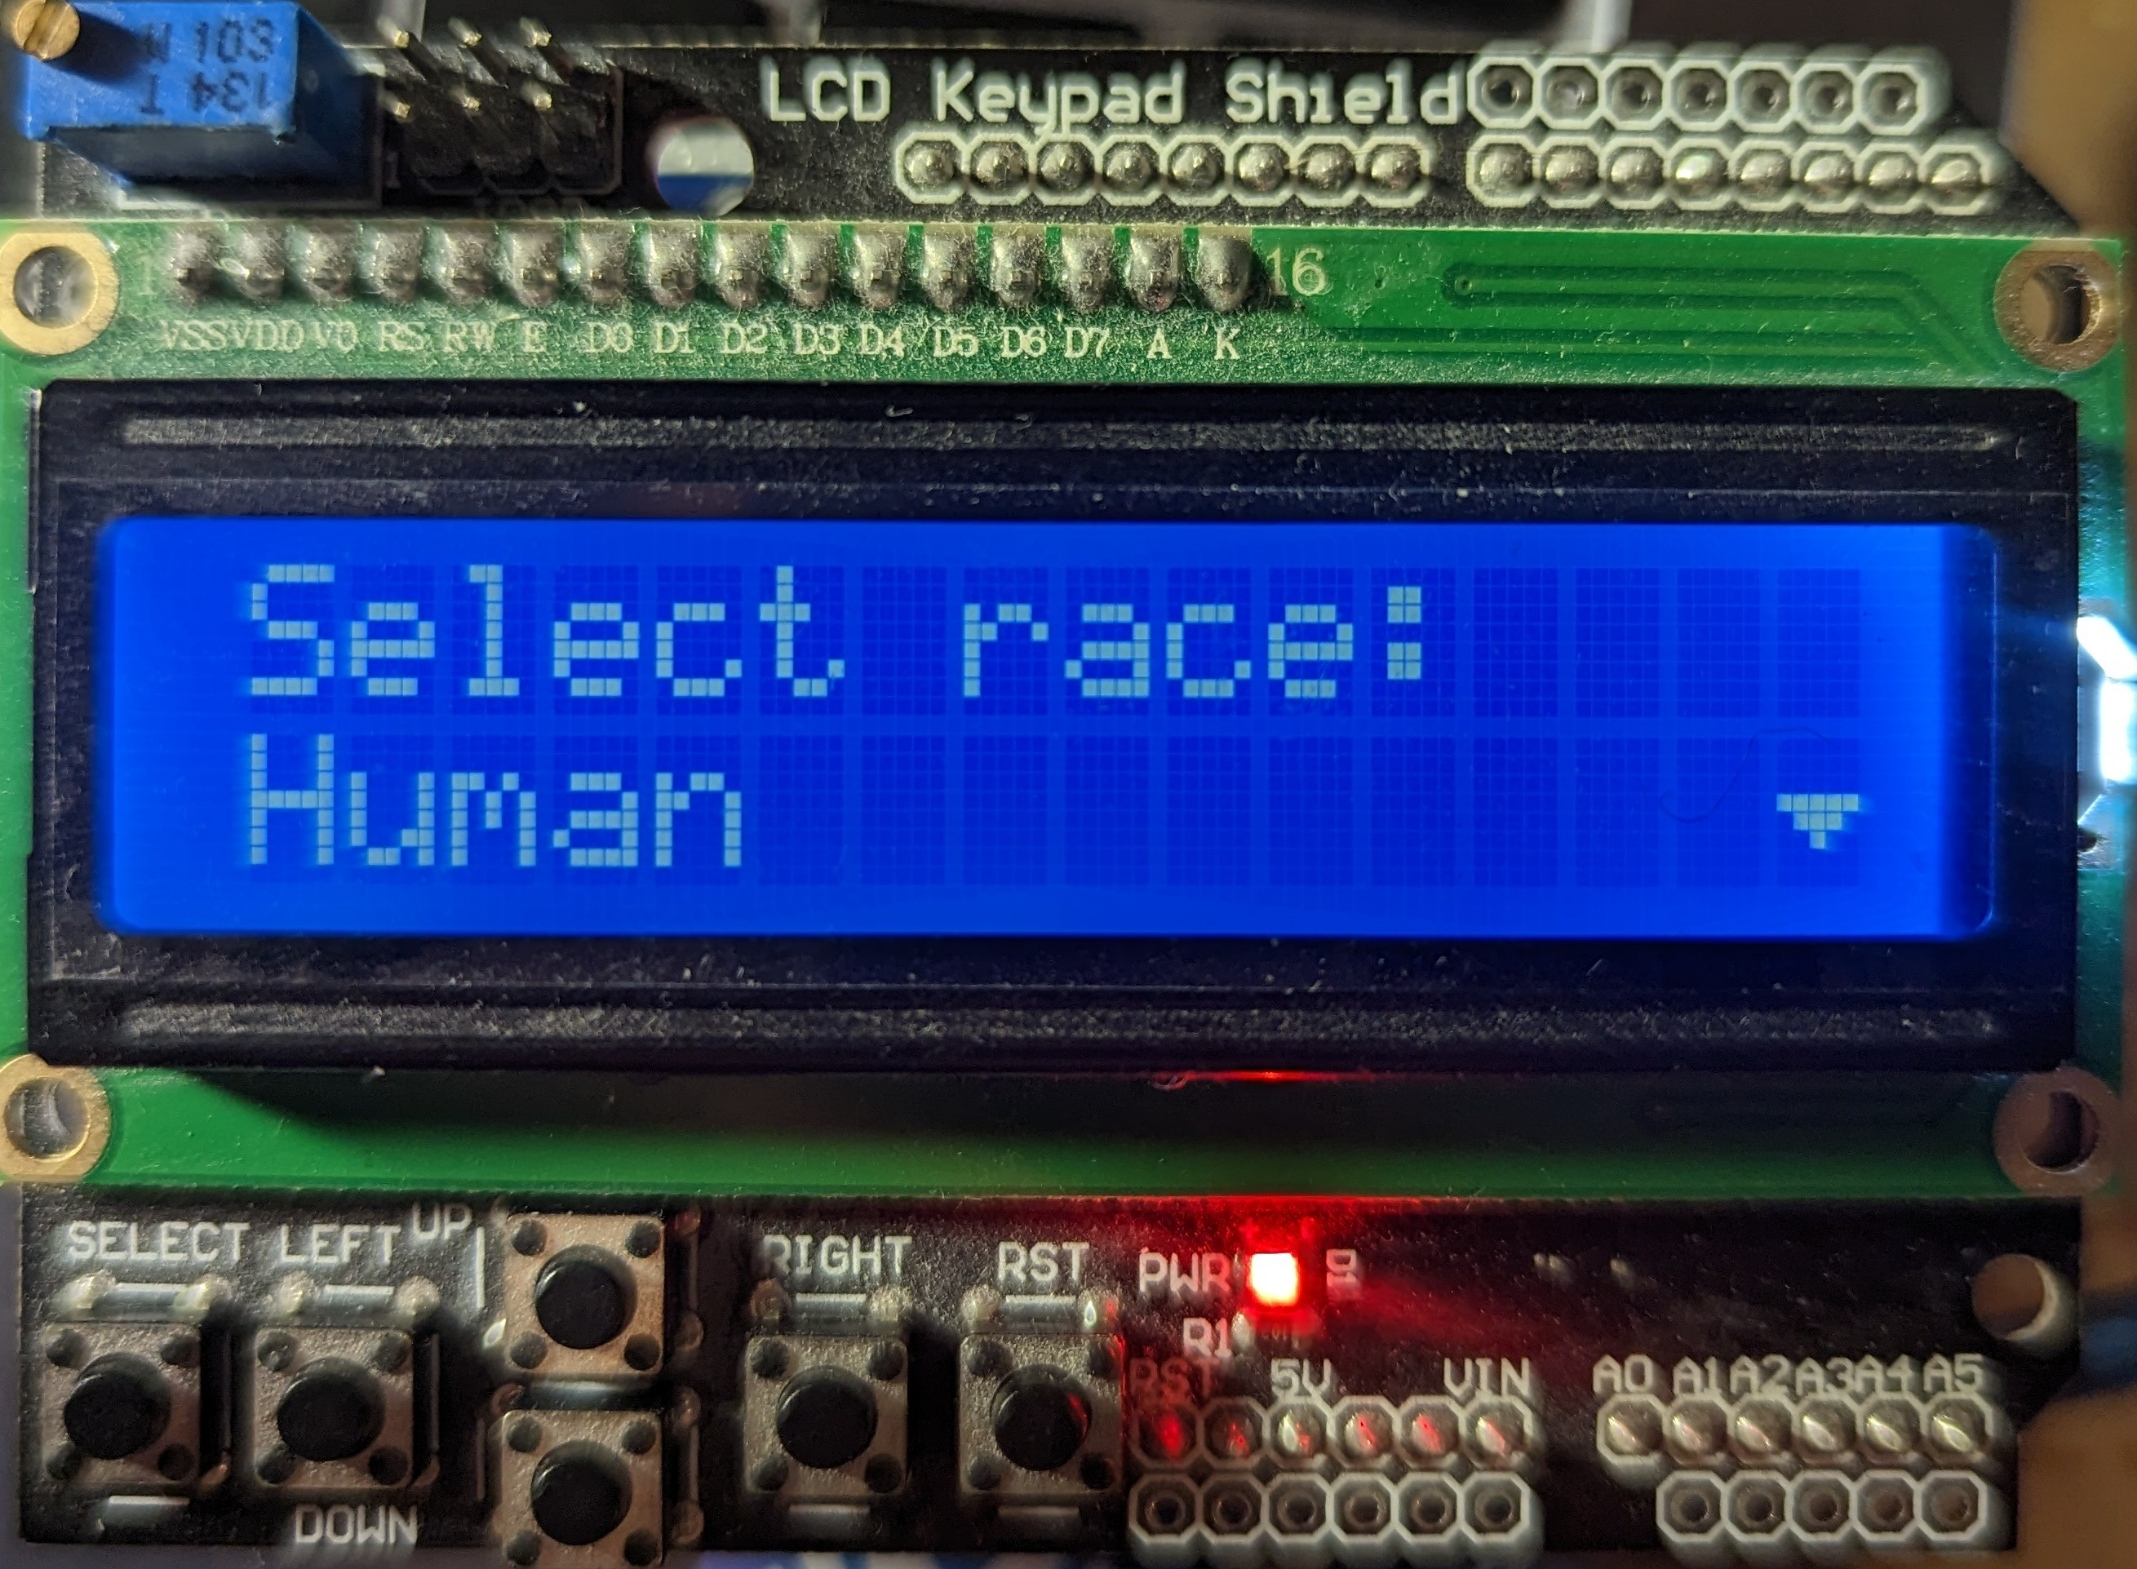
\includegraphics[width=1\linewidth]{selectRace.jpg}} \\
        \end{minipage}
        \vfill
        \begin{minipage}[h]{0.45\linewidth}
            \center{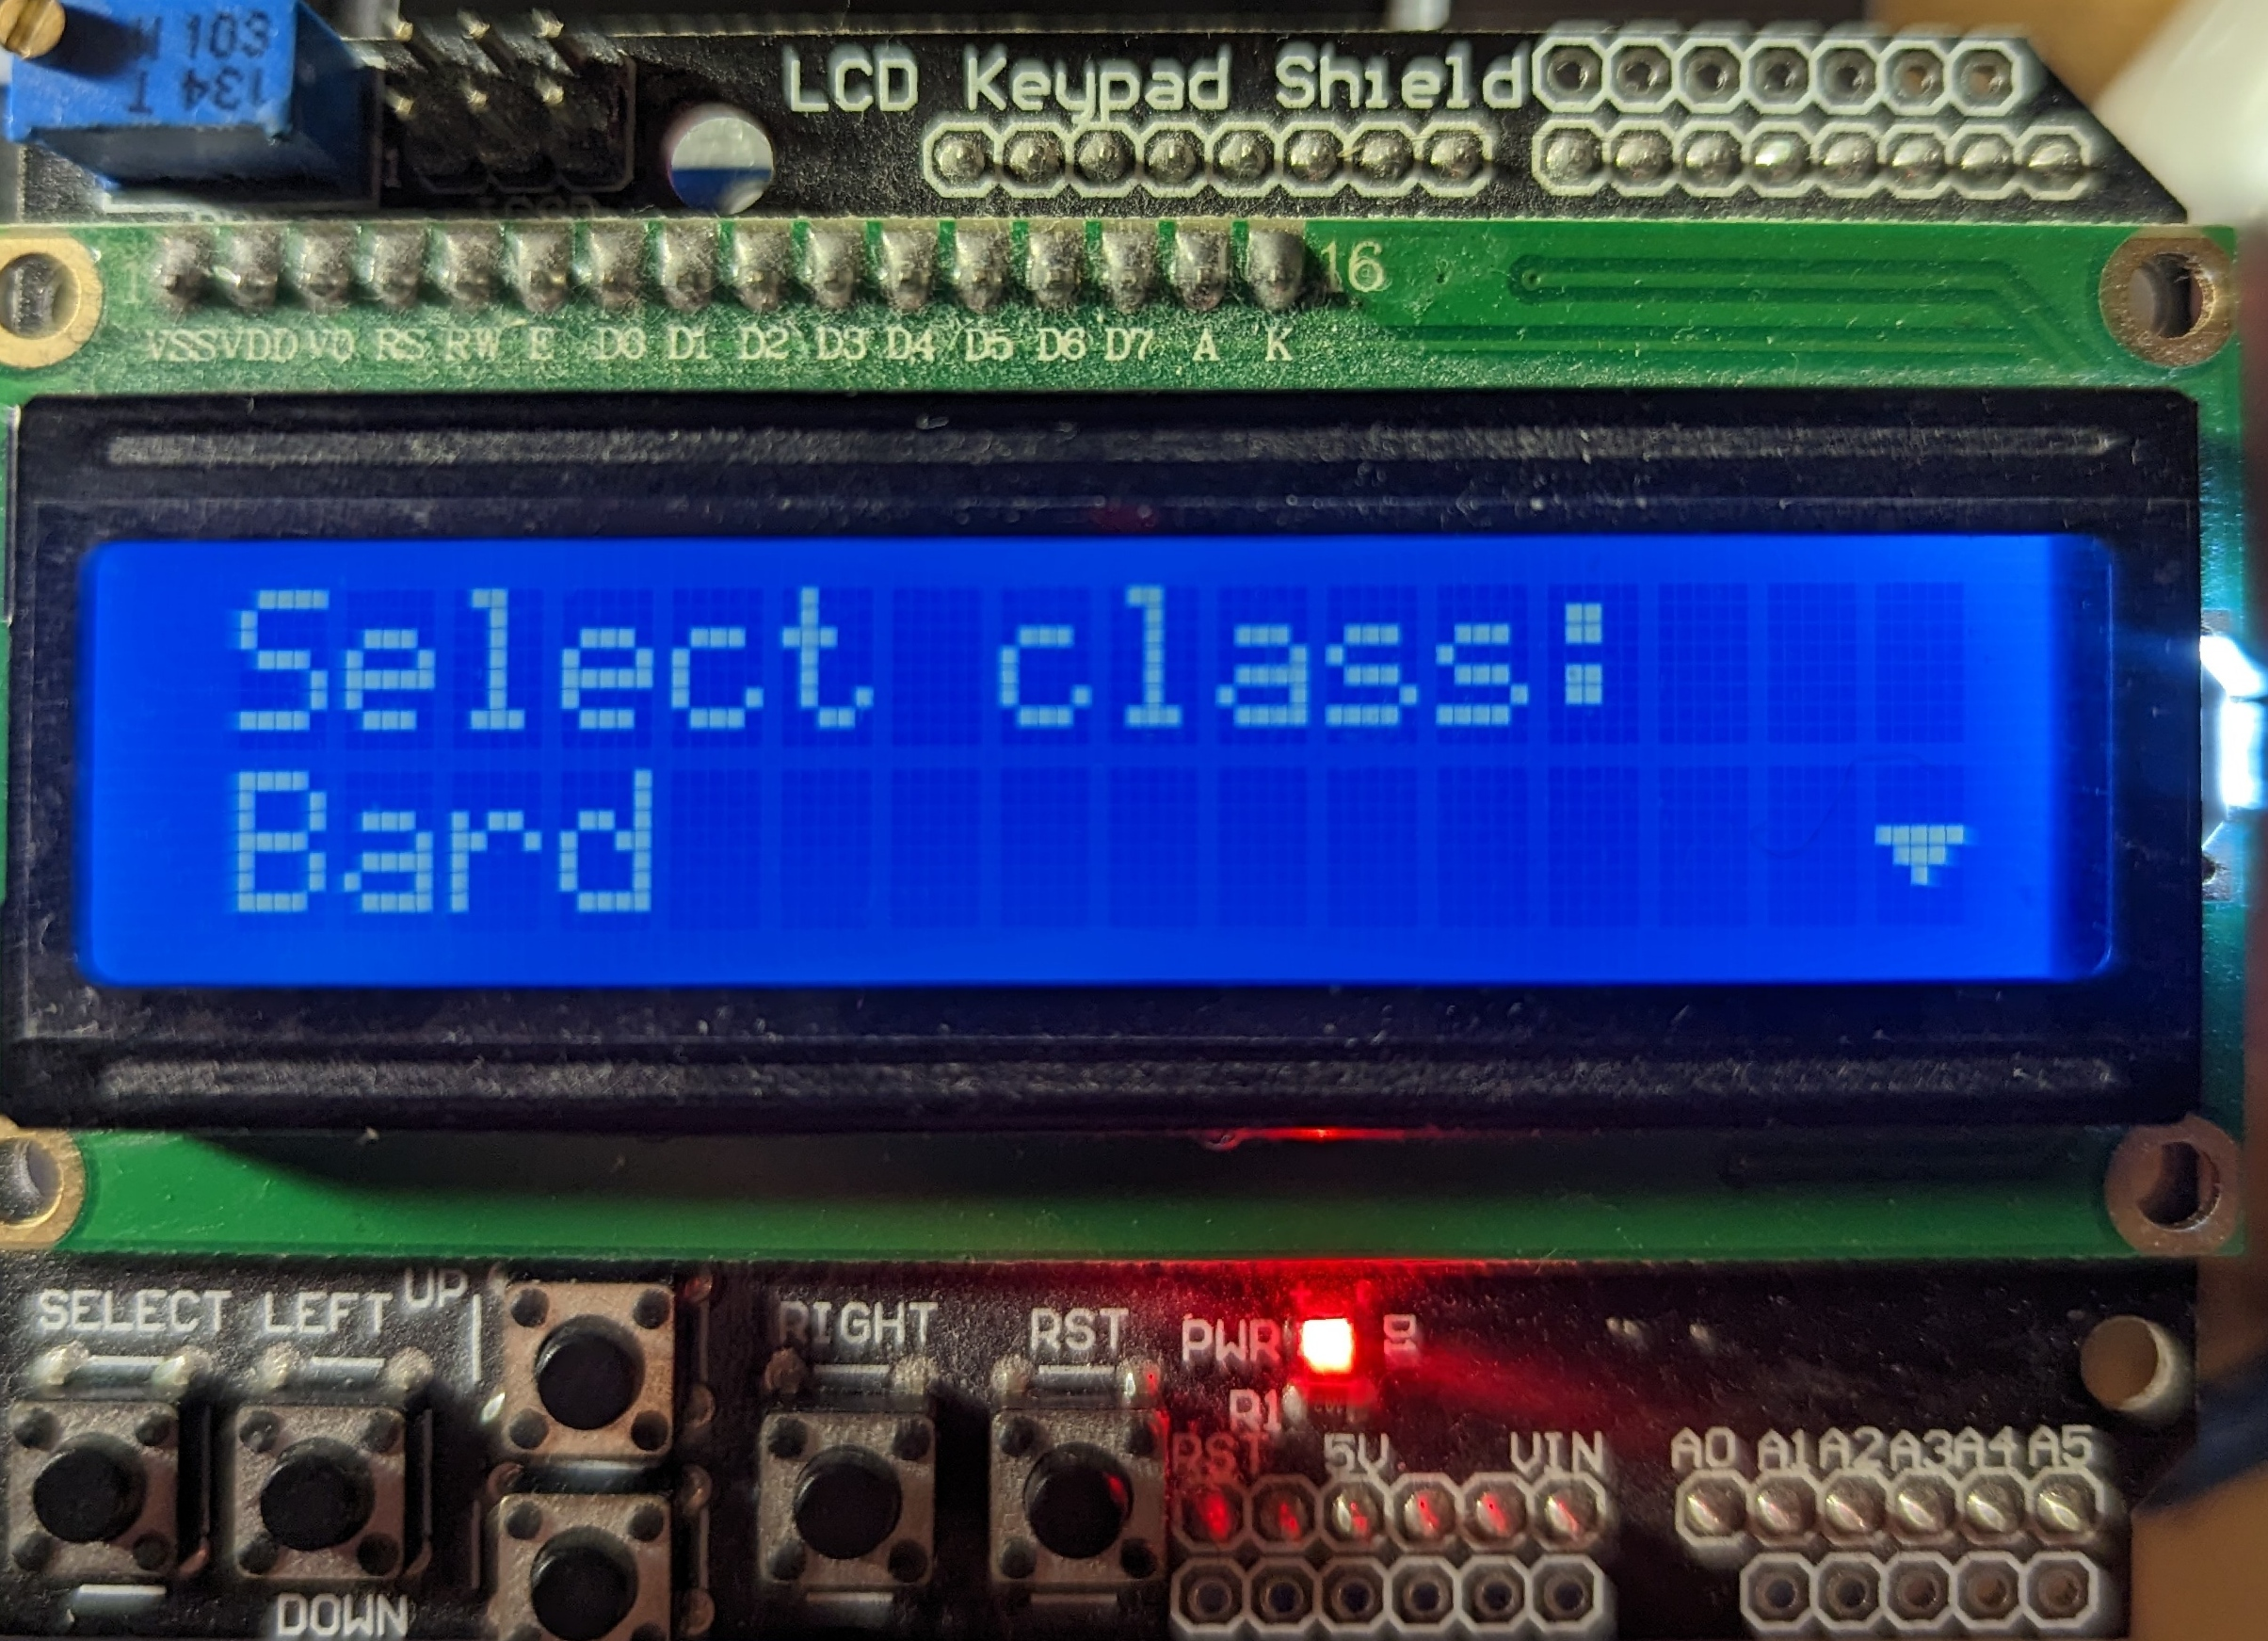
\includegraphics[width=1\linewidth]{selectClass.jpg}} \\
        \end{minipage}
        \hfill
        \begin{minipage}[h]{0.45\linewidth}
            \center{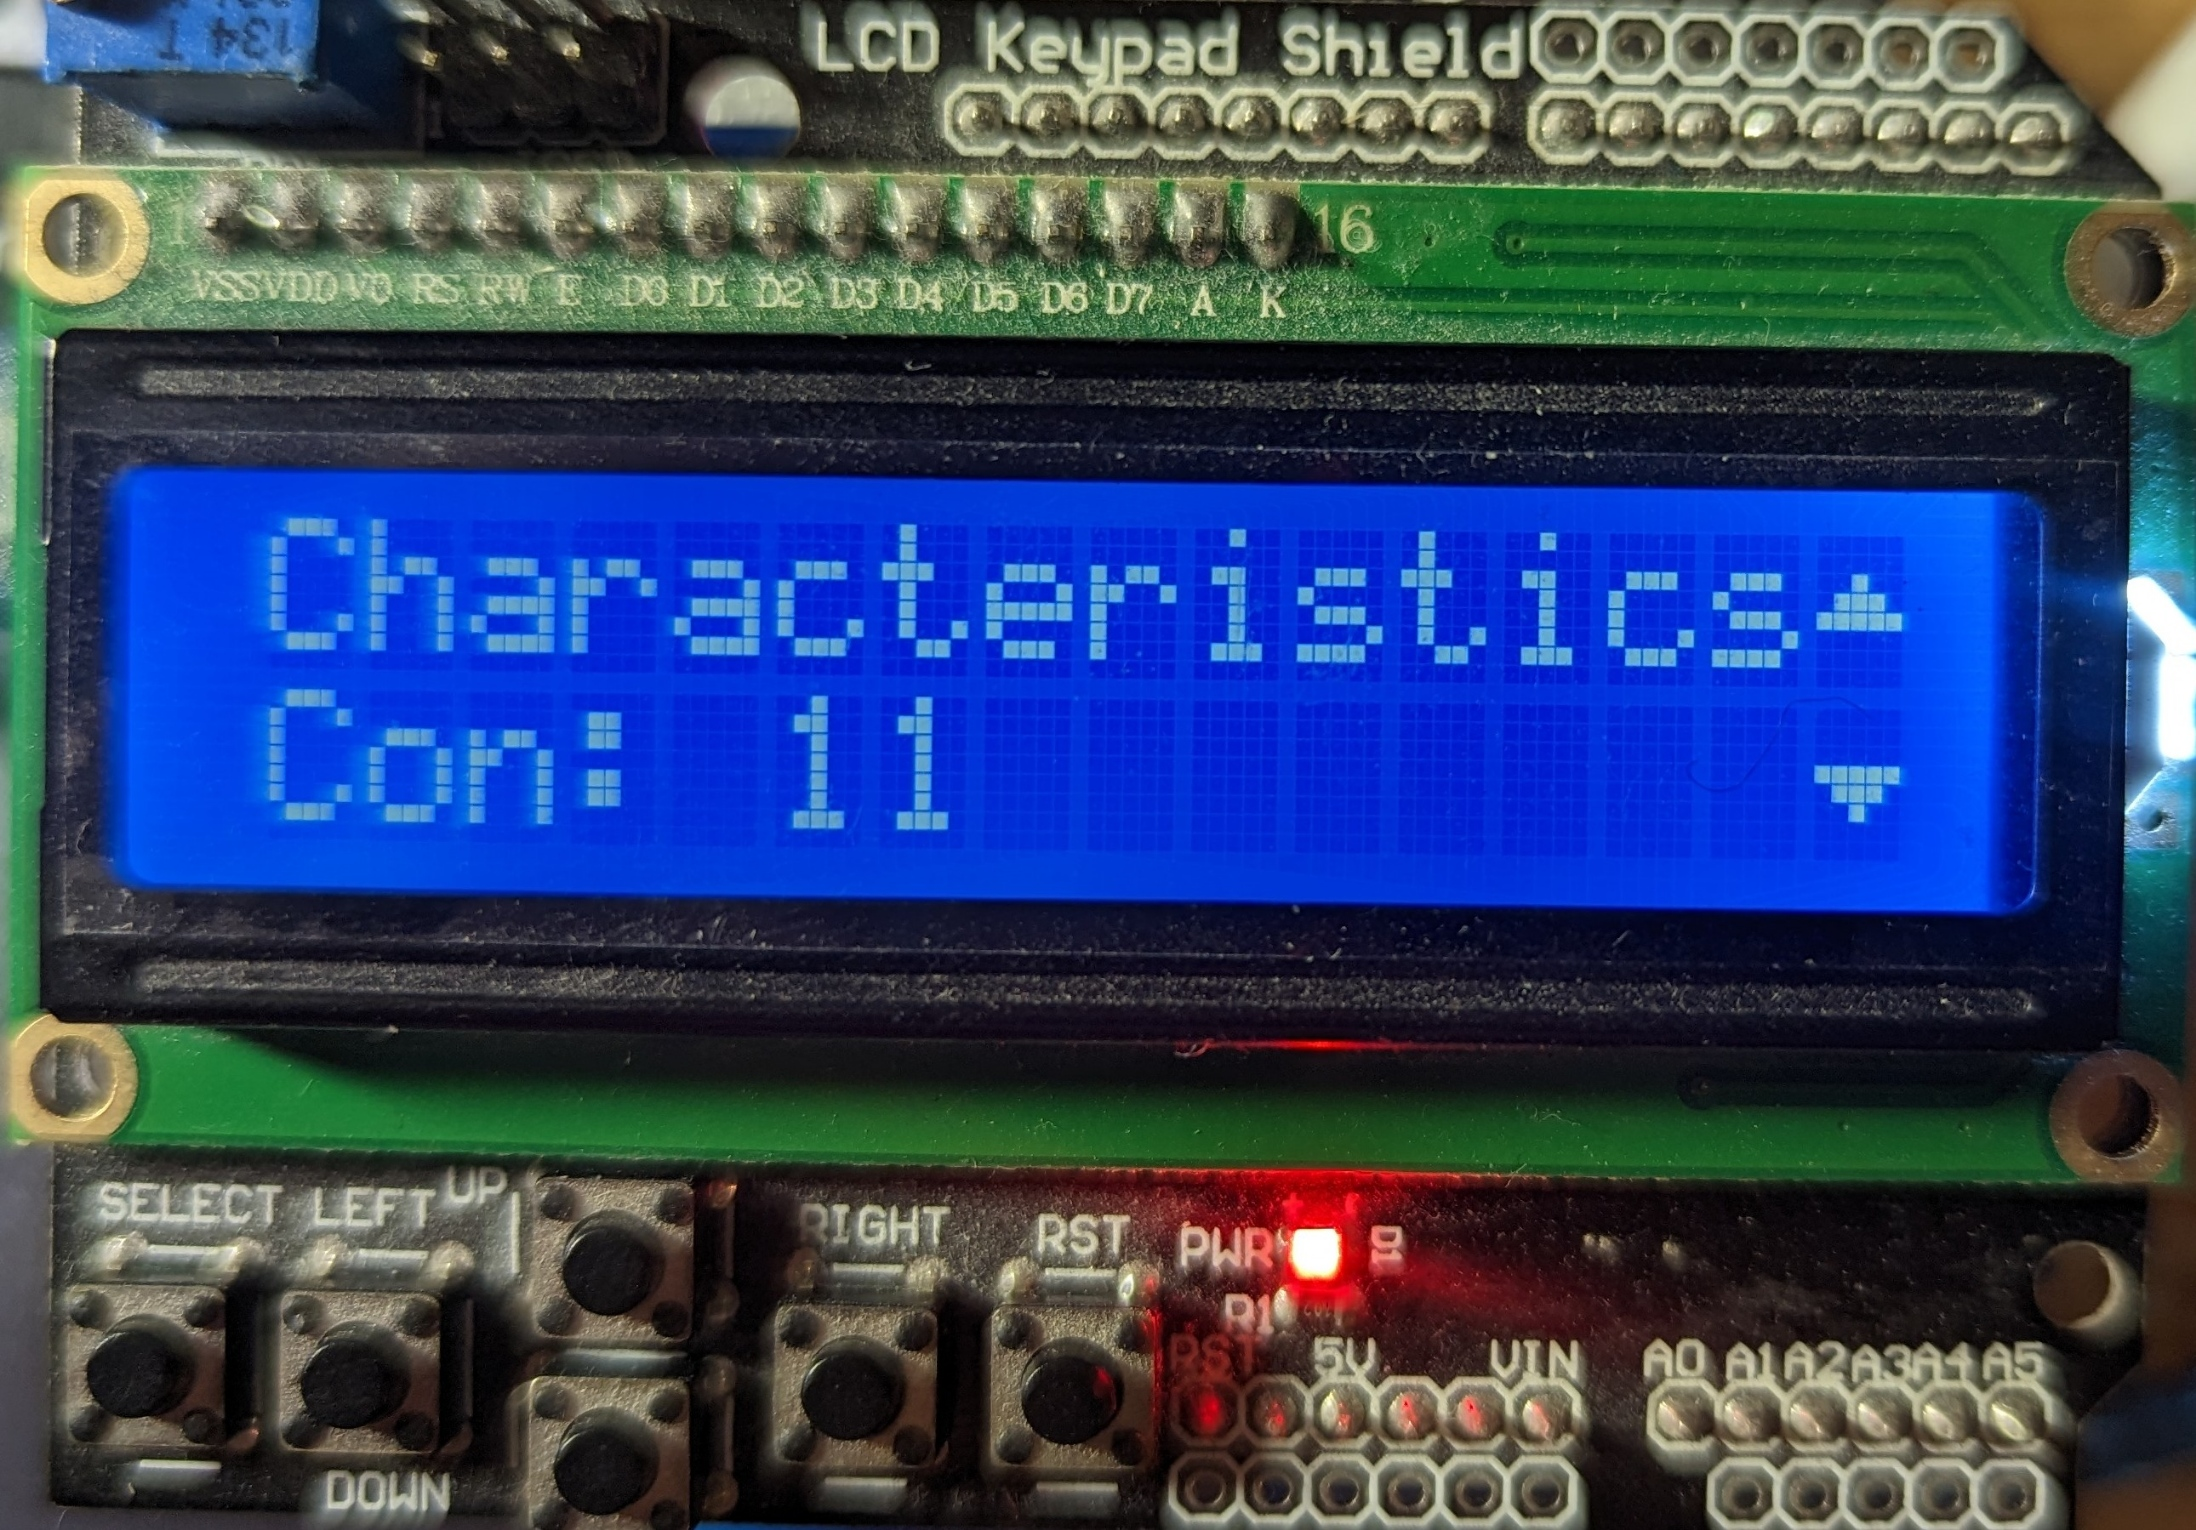
\includegraphics[width=1\linewidth]{output.jpg}} \\
        \end{minipage}
    \end{figure}
\end{frame}

\begin{frame}[fragile]{{\small Блок-схема алгоритма для выбора расы персонажа}}
\begin{figure}
        \centering
        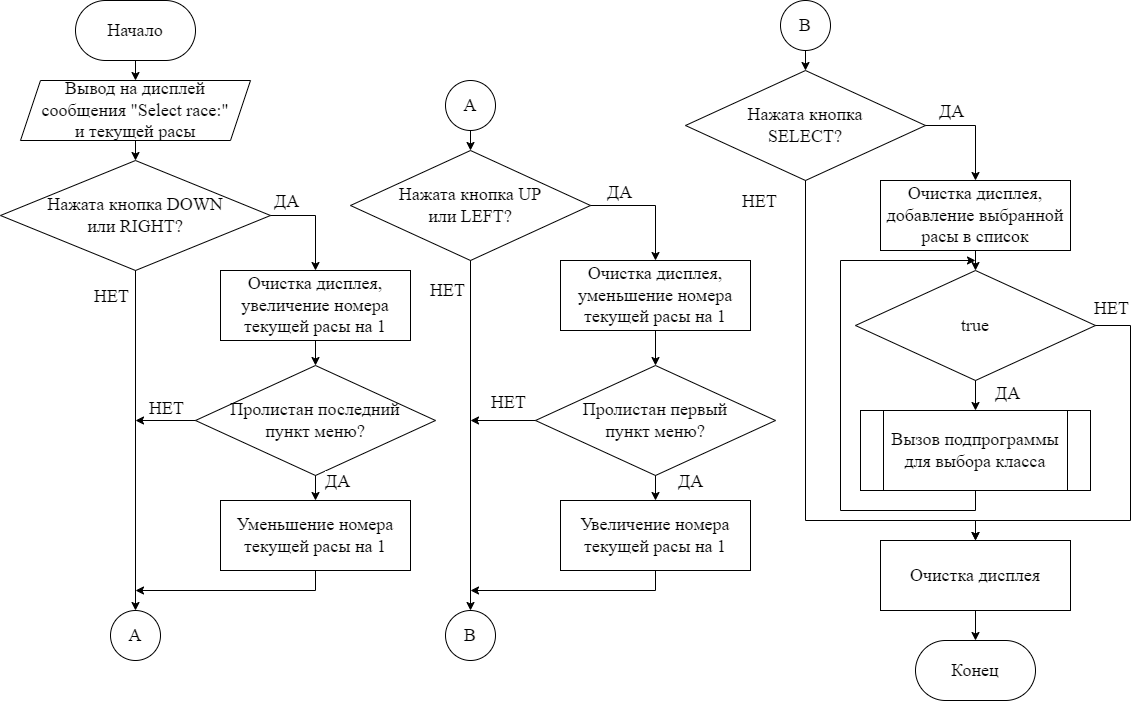
\includegraphics[width=\textwidth]{racePers.png}
        \label{fig:racePers}
    \end{figure}
\end{frame}

\newlength\someheight
\setlength\someheight{3,5cm}

\begin{frame}[fragile]{{\small Блок кода для выбора расы персонажа}}
    \begin{adjustbox}{width=\textwidth,height=\someheight,keepaspectratio}
    \begin{minipage}{1.1\linewidth}
    \begin{minted}{C++}
        if(i == 0) {    //  Верхний пункт меню
            lcd.print("Select race:");
            lcd.setCursor(0, 1);
            lcd.print(racePers[i]);
            lcd.createChar(2, arrowDown);
            lcd.setCursor(15, 1);
            lcd.print(char(2));
        } else if(i == 11) {    //  Нижний пункт меню
            lcd.print("Select race:");
            lcd.setCursor(0, 1);
            lcd.print(racePers[i]);
            lcd.createChar(1, arrowUp);
            lcd.setCursor(15, 0);
            lcd.print(char(1));
        } else {    //  Промежуточные пункты меню
            lcd.print("Select race:");
            lcd.setCursor(0, 1);
            lcd.print(racePers[i]);
            lcd.createChar(1, arrowUp);
            lcd.setCursor(15, 0);
            lcd.print(char(1));
            lcd.createChar(2, arrowDown);
            lcd.setCursor(15, 1);
            lcd.print(char(2));
        }
        delay(150);
        //  Обработка нажатия кнопок
        int btnRacePers = clickButton();
        switch (btnRacePers){
            case BTN_R:   //  Обработка нажатия кнопки RIGHT
                lcd.clear();
    \end{minted}
    \end{minipage}
    \hfill
    \begin{minipage}{1.1\linewidth}
    \begin{minted}{C++}
            i++;
            if (i > 11)
              i--;
            break;
          case BTN_U:   //  Обработка нажатия кнопки UP
            lcd.clear();
            i--;
            if (i < 0)
              i++;
            break;
          case BTN_D:   //  Обработка нажатия кнопки DOWN
            lcd.clear();
            i++;
            if (i > 11)
              i--;
            break;
          case BTN_L:   //  Обработка нажатия кнопки LEFT
            lcd.clear();
            i--;
            if (i < 0)
              i++;
            break;
          case BTN_S:   //  Обработка нажатия кнопки SELECT
            pers[0] = racePers[i];  //Запоминаем выбранную расу
            lcd.clear();
            while(true) {
              lcd.home();
              genClassPers(); //Вызываем функцию выбора класса
            }
            break;
          default:
            break;
          }
          lcd.clear();
    \end{minted}
    \end{minipage}
    \end{adjustbox}
\end{frame}

\begin{frame}[fragile]{{\small Блок кода для выбора класса персонажа}}
    \begin{adjustbox}{width=\textwidth,height=\someheight,keepaspectratio}
    \begin{minipage}{1.1\linewidth}
    \begin{minted}{C++}
        if(j == 0) {    //  Верхний пункт меню
          lcd.print("Select class:");
          lcd.setCursor(0, 1);
          lcd.print(classPers[j]);
          lcd.createChar(2, arrowDown);
          lcd.setCursor(15, 1);
          lcd.print(char(2));
        } else if(j == 12) {    //  Нижний пункт меню
          lcd.print("Select class:");
          lcd.setCursor(0, 1);
          lcd.print(classPers[j]);
          lcd.createChar(1, arrowUp);
          lcd.setCursor(15, 0);
          lcd.print(char(1));
        } else {    //  Промежуточные пункты меню
          lcd.print("Select class:");
          lcd.setCursor(0, 1);
          lcd.print(classPers[j]);
          lcd.createChar(1, arrowUp);
          lcd.setCursor(15, 0);
          lcd.print(char(1));
          lcd.createChar(2, arrowDown);
          lcd.setCursor(15, 1);
          lcd.print(char(2));
        }
        delay(150);
        //  Обработка нажатия кнопок
        int btnClassPers = clickButton();
        switch (btnClassPers){
          case BTN_R:   //  Обработка нажатия кнопки RIGHT
            lcd.clear();
    \end{minted}
    \end{minipage}
    \hfill
    \begin{minipage}{1.1\linewidth}
    \begin{minted}{C++}
            j++;
            if (j > 12)
              j--;
            break;
          case BTN_U:   //  Обработка нажатия кнопки UP
            lcd.clear();
            j--;
            if (j < 0)
              j++;
            break;
          case BTN_D:   //  Обработка нажатия кнопки DOWN
            lcd.clear();
            j++;
            if (j > 12)
              j--;
            break;
          case BTN_L:   //  Обработка нажатия кнопки LEFT
            lcd.clear();
            j--;
            if (j < 0)
              j++;
            break;
          case BTN_S:   //  Обработка нажатия кнопки SELECT
            pers[1] = classPers[j];
            lcd.clear();
            while(true) {
              lcd.home();
              charactPers();
            }
            break;
          default:
            break;
        }
        lcd.clear();
    \end{minted}
    \end{minipage}
    \end{adjustbox}
\end{frame}

\begin{frame}[fragile]{{\small Блок кода для генерации базовых характеристик персонажа}}
\begin{columns}
\begin{column}{0.35\textwidth}
\tiny
\begin{minted}[linenos,breaklines]{C++}
randomSeed(millis());
for (int i = 0; i < 6; i++) {
    roll = 6;
    characteristic = 0;
    for (int j = 0; j < 4; j++) {
        randRoll = random(1, 7);
        if (randRoll < roll) {
            roll = randRoll;
            characteristic += randRoll;
        } else {
            characteristic += randRoll;
        }
    }
    characteristics[i] = characteristic - roll;
}
\end{minted}
\end{column}
\begin{column}{0.65\textwidth}
    \begin{center}
     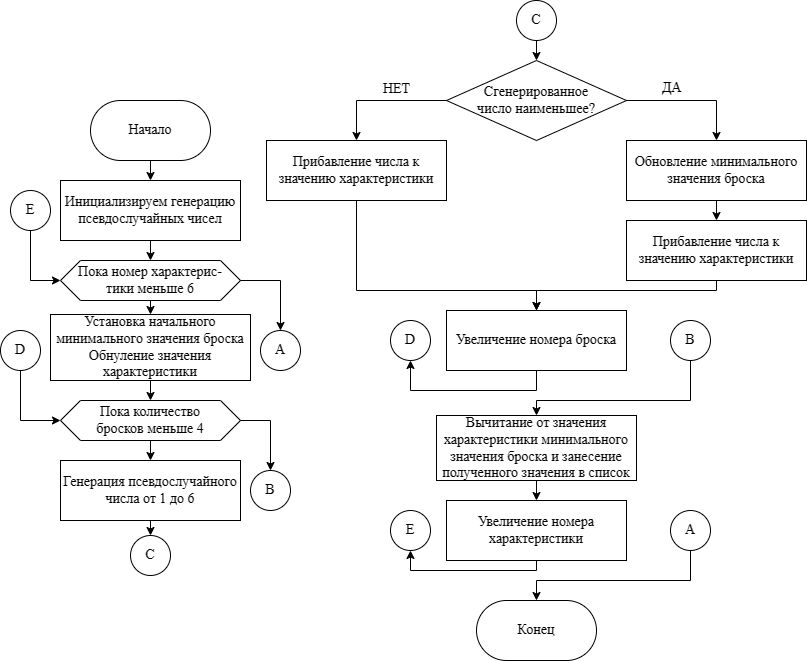
\includegraphics[width=\textwidth]{generate_character.png}
     \end{center}
\end{column}
\end{columns}
\end{frame}

\begin{frame}{Стоимость компонентов}
    \setlength{\parindent}{0.5cm}
    Для создания прототипа использовались следующие комплектующие:
    \begin{itemize}
        \item отладочная плата: Arduino Uno --- 1200 рублей;
        \item плата расширения: 1602 LCD Keypad Shield --- 860 рублей.
    \end{itemize}

    Итоговая стоимость компонентов составила: 2060 рублей.

    Стоимость компонентов по отдельности (без использования готовых отладочных плат и плат расширения):

    \begin{itemize}
        \item микроконтроллер ATmega 328 --- 162 рубля;
        \item LCD-дисплей 1602 --- 280 рублей;
        \item кнопки --- 8 рублей за 1 штуку.
    \end{itemize}
\end{frame}

\begin{frame}{Заключение}
    \setlength{\parindent}{0.5cm}
    В ходе выполнения работы были решены следующие задачи:

    \begin{enumerate}
        \item подобраны компоненты, необходимые для прототипирования генератора персонажей;
        
        \item спроектированы функциональные возможности приложения;
        
        \item реализованы в программном коде алгоритмы согласно базовым правилам D\&D5;
        
        \item отлажены и протестированы работоспособность программной и аппаратной части прототипа устройства;
        
        \item собран прототипа устройства.
    \end{enumerate}
    
    В результате выполнения работы было спроектировано и разработано устройство для генерации персонажа D\&D и все поставленные задачи были решены в полном объеме.
\end{frame}

\begin{frame}
    \centering Спасибо за внимание!
\end{frame}

\begin{frame}{Немного о Dungeons \& Dragons}
    \setlength{\parindent}{0.5cm}
    Основной целью игры Dungeons \& Dragons является описание персонажа и его приключений. Для создания персонажа могут быть задействованы игральные кости и Основные правила, а также личные предпочтения игроков.

    Основным средством для описания персонажа  служит лист персонажа -- сгруппированный в удобном виде набор характеристик персонажа. К таким характеристикам относятся следующие:

    \begin{enumerate}
        \item Основные атрибуты, присущие каждому персонажу: Сила, Телосложение, Ловкость, Интеллект, Мудрость, Харизма;
    
        \item Особые умения, которые индивидуализируют персонажа: способность к убеждению или расследованию;
    
        \item Определенные действия, такие как атака оружием или произнесение заклинаний;
    
        \item Языки, на которых говорит персонаж, или инструменты, которыми он умеет пользоваться.
    \end{enumerate}
\end{frame}

\begin{frame}{\smallПравила для генерации базовых характеристик персонажа}
    \setlength{\parindent}{0.5cm}
    Персонаж обладает шестью характеристиками: Сила, Телосложение, Ловкость, Интеллект, Мудрость и Харизма.
    
    Есть несколько способов для генерации:

    \begin{enumerate}
        \item 3d6 -- классический способ, генерация осуществляется броском 3d6 (трёхкратным броском шестигранного кубика).

        \item 4d6 -- один из альтернативных способов, генерация осуществляется броском 4d6 (четырехкратным броском игральной кости), а минимальное значение среди бросков отбрасывается.

        \item Персонаж начинает со всеми характеристикам равными 8. У игрока есть 27 очков, которые он может свободно распределить, при этом 14 и 15 значение характеристики стоят по 2 очка каждое.

        \item В D\&D 5e основной метод определения характеристик -- выбор из набора стандартных значений: 15, 14, 13, 12, 10, 8.
    \end{enumerate}
\end{frame}

\begin{frame}{Выбор расы и класса персонажа}
    \setlength{\parindent}{0.5cm}
    Каждый персонаж принадлежит расе -- виду, в мире фэнтези. Самые общие игровые расы -- это дварфы, эльфы, халфлинги и люди. Существует еще много иных рас, которые могут быть доступны на усмотрение Мастера.
    
    Раса персонажа, в частности определяет его расовые черты, такие как корректировка очков характеристик, особые чувства, талант к использованию определенного оружия, или способность использовать малые заклинания. Иногда эти черты соответствуют возможностям определенных классов.
    
    Каждый персонаж также -- член класса. Самые распространенные классы -- это жрец, боец, разбойник и маг. Другие классы могут быть доступны на усмотрение Мастера.
    
    Персонаж также получает некоторые преимущества от выбранного класса. Многие из этих преимуществ это особенности класса, отличающие его от остальных.
\end{frame}
\end{document}
